\documentclass[11pt]{article}
\usepackage{geometry}
\usepackage[utf8]{inputenc}
\usepackage[english]{babel}
\usepackage{amsmath}
\usepackage{amssymb}
\usepackage{amsfonts}
\usepackage[
    pdftex, 
    dvipsnames
]{xcolor}
\usepackage[
    colorlinks=true,
    linkcolor=black,
    urlcolor=Thistle
]{hyperref}
\usepackage{fancyhdr}
\usepackage{datetime}
\usepackage{xargs}
\usepackage{ccicons}
\usepackage{mdframed}
\usepackage{caption}
\usepackage{cancel}
\usepackage[nottoc]{tocbibind}
\usepackage[
    outputdir=.texpadtmp
]{minted}

% ==== License =====
\usepackage[
    type={CC}, 
    modifier={by-nc-sa}, 
    version={4.0},
]{doclicense}

% ==== todo notes ====
\usepackage[
    colorinlistoftodos,
    prependcaption,
    textsize=tiny
]{todonotes}
\newcommandx{\note}[2][1=]{\todo[linecolor=Thistle,backgroundcolor=Thistle!25,bordercolor=Thistle,#1]{#2}}
\newcommandx{\unsure}[2][1=]{\todo[linecolor=red,backgroundcolor=red!25,bordercolor=red,#1]{#2}}
\newcommandx{\change}[2][1=]{\todo[linecolor=blue,backgroundcolor=blue!25,bordercolor=blue,#1]{#2}}
\newcommandx{\info}[2][1=]{\todo[linecolor=OliveGreen,backgroundcolor=OliveGreen!25,bordercolor=OliveGreen,#1]{#2}}

% General
\newcommand{\mc}[1]{\mathcal{#1}}

% Math Bold Font, Vector Notations
\newcommand{\ba}{\mathbf{a}}
\newcommand{\bb}{\mathbf{b}}
\newcommand{\bc}{\mathbf{c}}
\newcommand{\bd}{\mathbf{d}}
\newcommand{\be}{\mathbf{e}}
\renewcommand{\bf}{\mathbf{f}}
\newcommand{\bg}{\mathbf{g}}
\newcommand{\bh}{\mathbf{h}}
\newcommand{\bi}{\mathbf{i}}
\newcommand{\bj}{\mathbf{j}}
\newcommand{\bk}{\mathbf{k}}
\newcommand{\bl}{\mathbf{l}}
\newcommand{\bm}{\mathbf{m}}
\newcommand{\bn}{\mathbf{n}}
\newcommand{\bo}{\mathbf{o}}
\newcommand{\bp}{\mathbf{p}}
\newcommand{\bq}{\mathbf{q}}
\newcommand{\br}{\mathbf{r}}
\newcommand{\bs}{\mathbf{s}}
\newcommand{\bt}{\mathbf{t}}
\newcommand{\bu}{\mathbf{u}}
\newcommand{\bv}{\mathbf{v}}
\newcommand{\bw}{\mathbf{w}}
\newcommand{\bx}{\mathbf{x}}
\newcommand{\by}{\mathbf{y}}
\newcommand{\bz}{\mathbf{z}}
\newcommand{\bzero}{\mathbf{0}}

% Proofs, Structures
\newcommand{\proof}{\tit{\underline{Proof:}}} % This equivalent to the \begin{proof}\end{proof} block
\newcommand{\proofforward}{\tit{\underline{Proof($\implies$):}}}
\newcommand{\proofback}{\tit{\underline{Proof($\impliedby$):}}}
\newcommand{\proofsuperset}{\tit{\underline{Proof($\supseteq$):}}}
\newcommand{\proofsubset}{\tit{\underline{Proof($\subseteq$):}}}
\newcommand{\contradiction}{$\longrightarrow\!\longleftarrow$}
\newcommand{\qed}{\hfill $\blacksquare$}

% Number Spaces, Vector Space
\newcommand{\R}{\mathbb{R}}
\newcommand{\real}{\mathbb{R}}
\newcommand{\complex}{\mathbb{C}}
\newcommand{\field}{\mathbb{F}}

% customized commands
\newcommand{\settag}[1]{\renewcommand{\theenumi}{#1}}
\newcommand{\tbf}[1]{\textbf{#1}}
\newcommand{\tit}[1]{\textit{#1}}
\newcommand{\overbar}[1]{\mkern 1.5mu\overline{\mkern-1.5mu#1\mkern-1.5mu}\mkern 1.5mu}
\newcommand{\double}[1]{\mathbb{#1}} % Set to behave like that on word
\newcommand{\trans}[3]{$#1:#2\rightarrow{}#3$}
\newcommand{\map}[3]{\text{$\left[#1\right]_{#2}^{#3}$}}
\newcommand{\dime}[1]{\mathrm{dim}(#1)}
\newcommand{\mat}[2]{M_{#1 \times #2}(\R)}
\newcommand{\aug}{\fboxsep=-\fboxrule\!\!\!\fbox{\strut}\!\!\!}
\newcommand{\basecase}{\textsc{\underline{Basis Case:}} }
\newcommand{\inductive}{\textsc{\underline{Inductive Step:}} }
\newcommand{\norm}[1]{\left\lVert#1\right\rVert}
\newcommand{\independent}{\perp \!\!\! \perp}

% Set section number in front of equation enumerations
\counterwithin{equation}{section}
\counterwithin{footnote}{section}
\author{\ccLogo\,\, Tingfeng Xia}
\title{\textsc{CSC317/418 Computer Graphics}}
\date{Winter Term, 2021}

\begin{document}
\maketitle
\doclicenseThis
\section*{Information}
\begin{itemize}
	\item Starting winter term 2021, Computer Graphics will be switching from its previous course code CSC418 to CSC317. 
	\item Course webpage: \url{https://github.com/karansher/computer-graphics-csc317}
	\item This note contains figures from Prof. Karan Singh's lecture slides. It also might contain figures by Marschner and Shirley and David Levin. 
	\item Textbook: Shirley, P., \& Marschner, S. (2009). \textit{Fundamentals of Computer Graphics (Third Edition)}. 
\end{itemize}
\tableofcontents
\section{Raster Image} This section will be added later. 
\section{Ray Casting} This section will be added later. 
\section{Ray Tracing}
\subsection{Light and Surfaces}
There are two types of lights, namely directional and point light sources. 
\begin{itemize}
	\item The directional light has its light direction independent of the object, this typically happens when the light is very far away. (e.g. the sun)
	\item On the other hand, point light are such that the direction of light depends on position of object relative to light. Think of this as a light bulb in a room. 
\end{itemize}
\subsection{Shading}
The goal of shading is to compute the light reflected toward camera. As an algorithm it expects the following inputs: eye direction, light direction for each of many lights, surface normal, and surface parameters such as color and shininess. 

\paragraph{The Surface Normal} at a hit point can be computed, depending on the type of specification
\begin{itemize}
	\item Polygon normal: cross product of two non-collinear edges, 
	\item Implicit surface normal $f(p) = 0$: $gradient(f)(p)$
	\item Explicit parametric surface $f(a,b)$: 
	\begin{equation}
		\frac{\partial f(s, b)}{\partial s} \times \frac{\partial f(a, t)}{\partial t}
	\end{equation}
\end{itemize}

\subsection{Light Falloff}
The light falloff aims to model the concept of diminishing light intensity based on distance. Suppose the light source has intensity of $I$, then, at a point that is $r$ (Euclidean Distance) away from the light source, the light intensity from that particular light source would be
\begin{equation}
	\text{Intensity}(I, r) = I / r^2
\end{equation}
Clearly, when we are at the light source, $r = 0$ and we attain the max intensity. 

\subsection{Diffuse Reflection}
In the case of diffuse reflection, light are scattered uniformly in all directions, i.e. he surface color is the same for all viewing directions. The amount of light captured by a surface obeys Lamber's cosine law. (We call this Lambertian surface.) Figure \ref{lambert} illustrates the relationship. 

\begin{figure}
	\centering 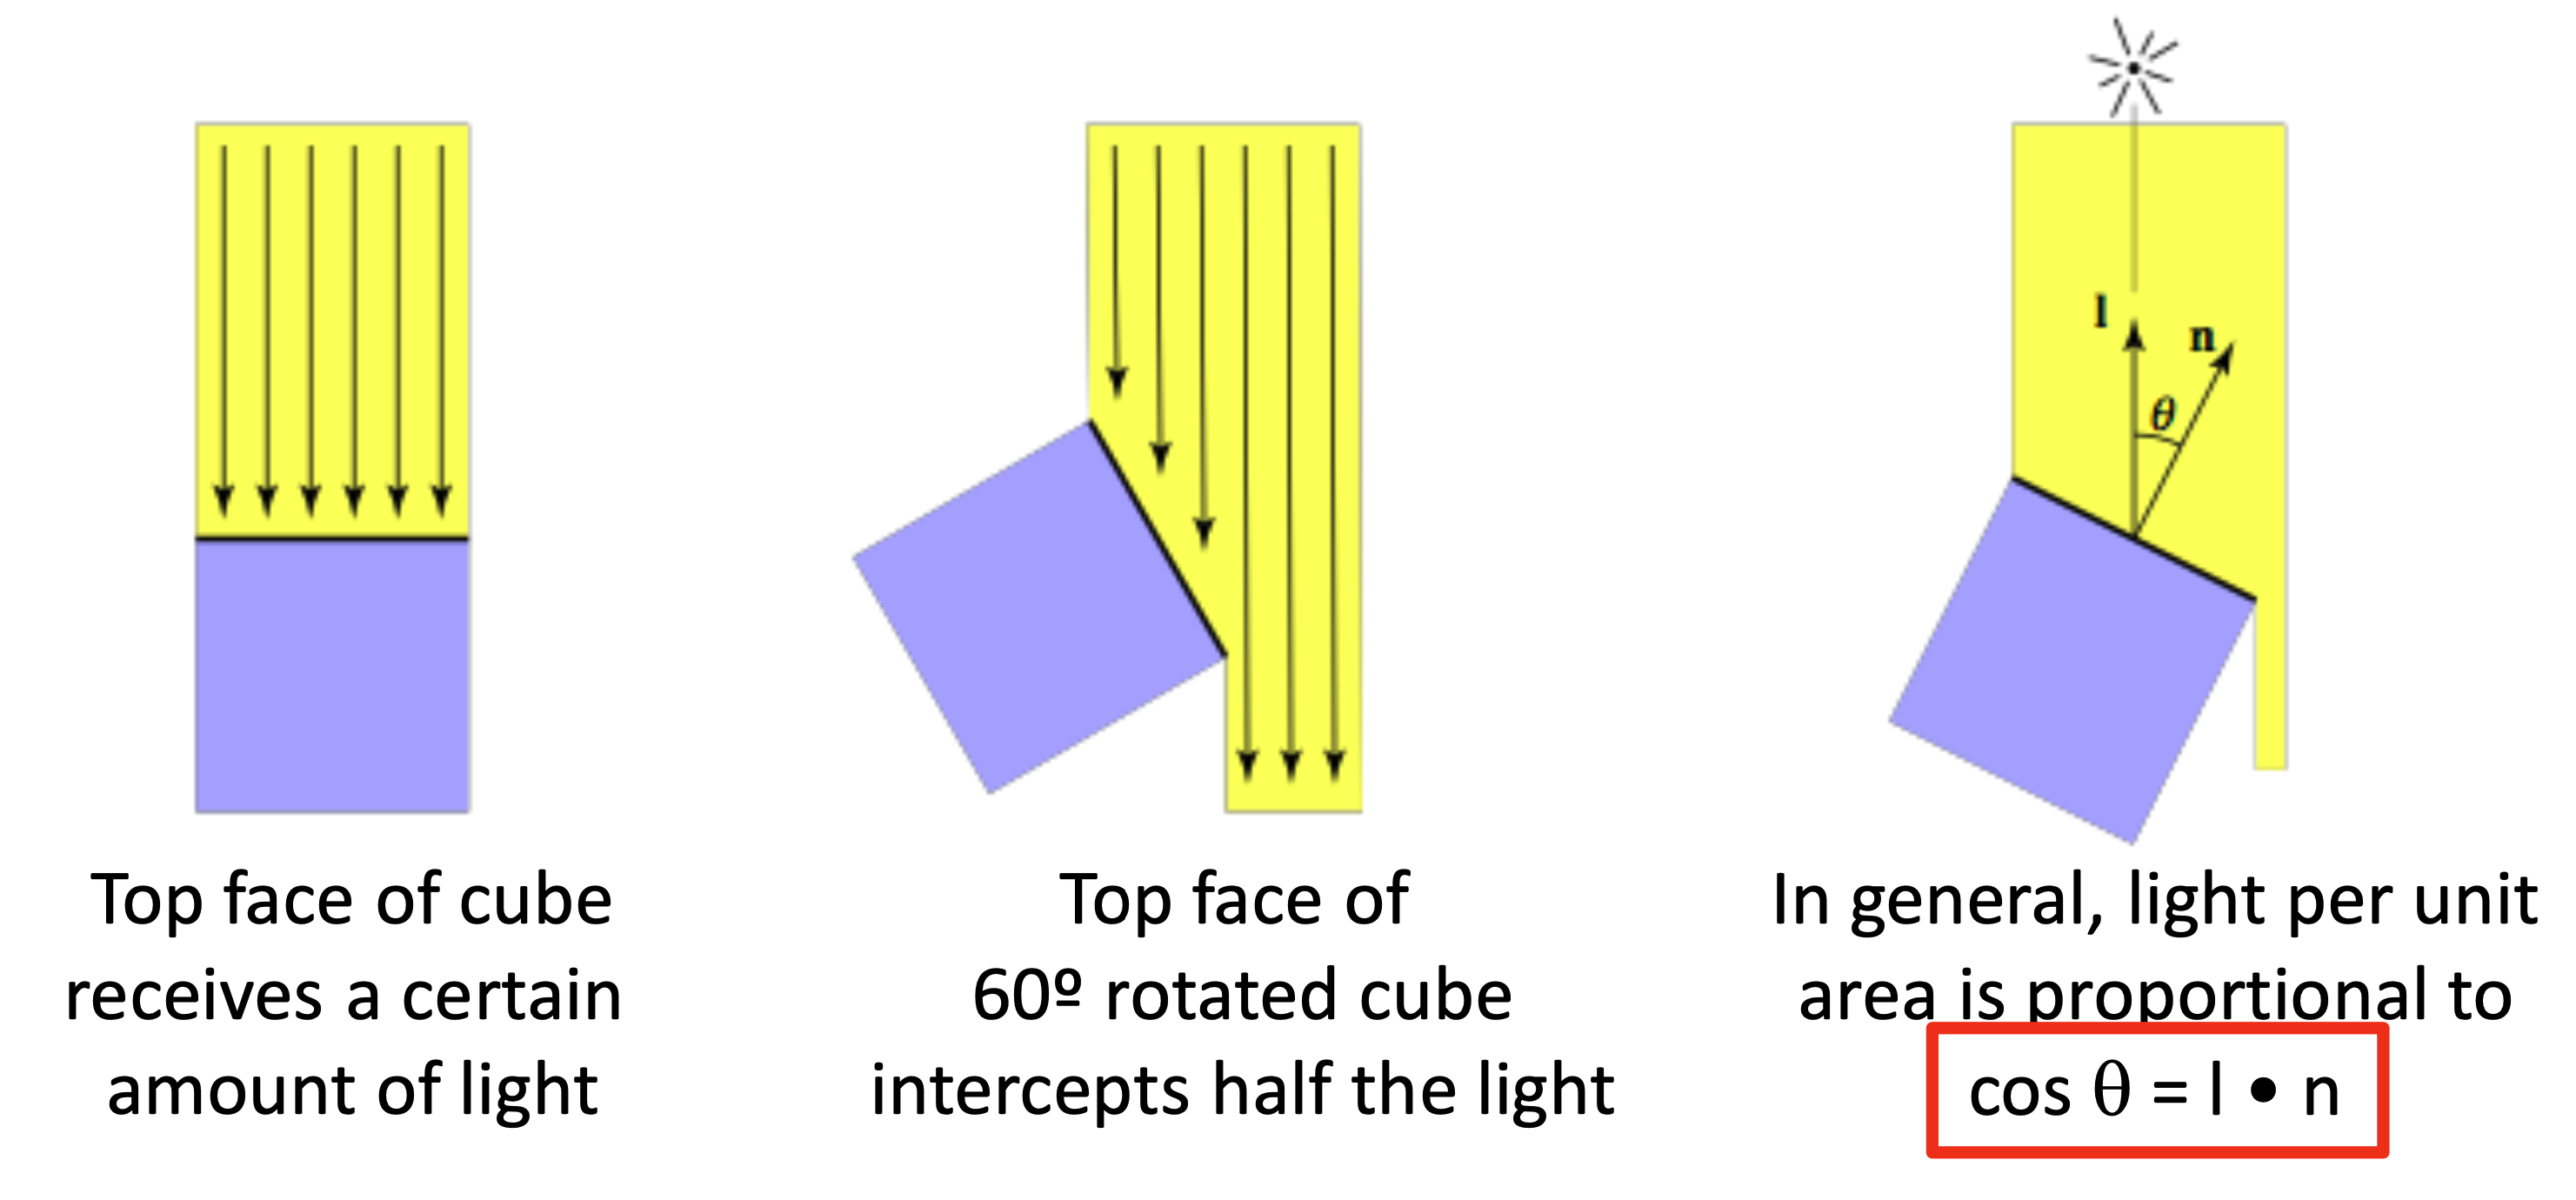
\includegraphics[width=0.7\textwidth]{figs/lambert}
	\caption{\label{lambert} Illustration of Lambert's cosine law. }
\end{figure}

\subsection{Lambertian Shading} 
The Lambertian Shading is independent of view direction. Let's call $L_d:=$ diffusely reflected light, $k_d:=$ diffuse coefficient\note{$k_d$ could be separate for three color channels. }, and $I:=$ illumination from source, then 
\begin{equation}
	L_{d}=k_{d}\circ \left(I / r^{2}\right) \max (0, \mathbf{n} \cdot \mathbf{l})
\end{equation}
This produces a matte appearance. 

\subsection{Shadows}
Surface is only illuminated if nothing blocks its view of the light. With ray tracing it's easy to check if a point in the scene is in shadow, all you have to do is just shoot a ray from the point\footnote{This ``point'' means the actual location in 3d of what a pixel on the image projects to. } to the light and intersect it with the scene.

\subsection{Multiple Light Sources}
\begin{itemize}
	\item Important to fill in black shadows, 
	\item and just loop over lights, add contributions
	\item Ambient shading
	\begin{itemize}
		\item Black shadows are not really right, 
		\item easy solution: dim light at the camera, so everything we see must  be lit up (might be dim, but not black)
		\item alternative: add a constant ambient color to the shading. 
	\end{itemize}
\end{itemize}

\subsection{Ambient Shading}
Ambient shading are those that does not depend on anything, we add a constant color to account for disregarded illumination and fill in black shadows. Let's call $L_a:=$ reflected ambient light, $k_a:=$ ambient coefficient\note{This $k_a$ could again be separate for different color channels}, and $I_a$ the raw light intensity, then
\begin{equation}
	L_a = k_a \circ I_a
\end{equation}

\subsection{Algorithm Template}
Let's present the algorithm template for images with multiple light sources here
\begin{mdframed}
	\begin{minted}{cpp}
shade(ray, lights, point, normal) {
    result = ambient; 
    for light in lights {
        I = light.pos - position; 
        shadowray = (point + eps * normal, I); 
        if !scene.intersection(result, shadowray) {
            it = surface.k * light.intensity * max(0, normal.dot(I));
            result += surface.color * it;
        }
    }
    return result; 
}
	\end{minted}
\end{mdframed}
Do notice that we have \texttt{shadowray = (point + eps * normal, I);}, and the eps is there to prevent floating point numerical errors. If we don't do that it is possible a ray would intersect immediately with the surface, and produce unusable images. 

\subsection{Mirror Reflection}
Now we've talked about diffuse reflections (matte surfaces), let's see the case of mirror reflection. We discuss the case of imperfect mirror here, where the intensity depends on view direction - reflects incident light from mirror direction. Figure \ref{mirror reflection} illustrates the scenario. The reflected ray vector is 
\begin{equation}
	\br = 2 (\bn \cdot \bl) \bn - \bl
\end{equation}
\begin{figure}
	\centering 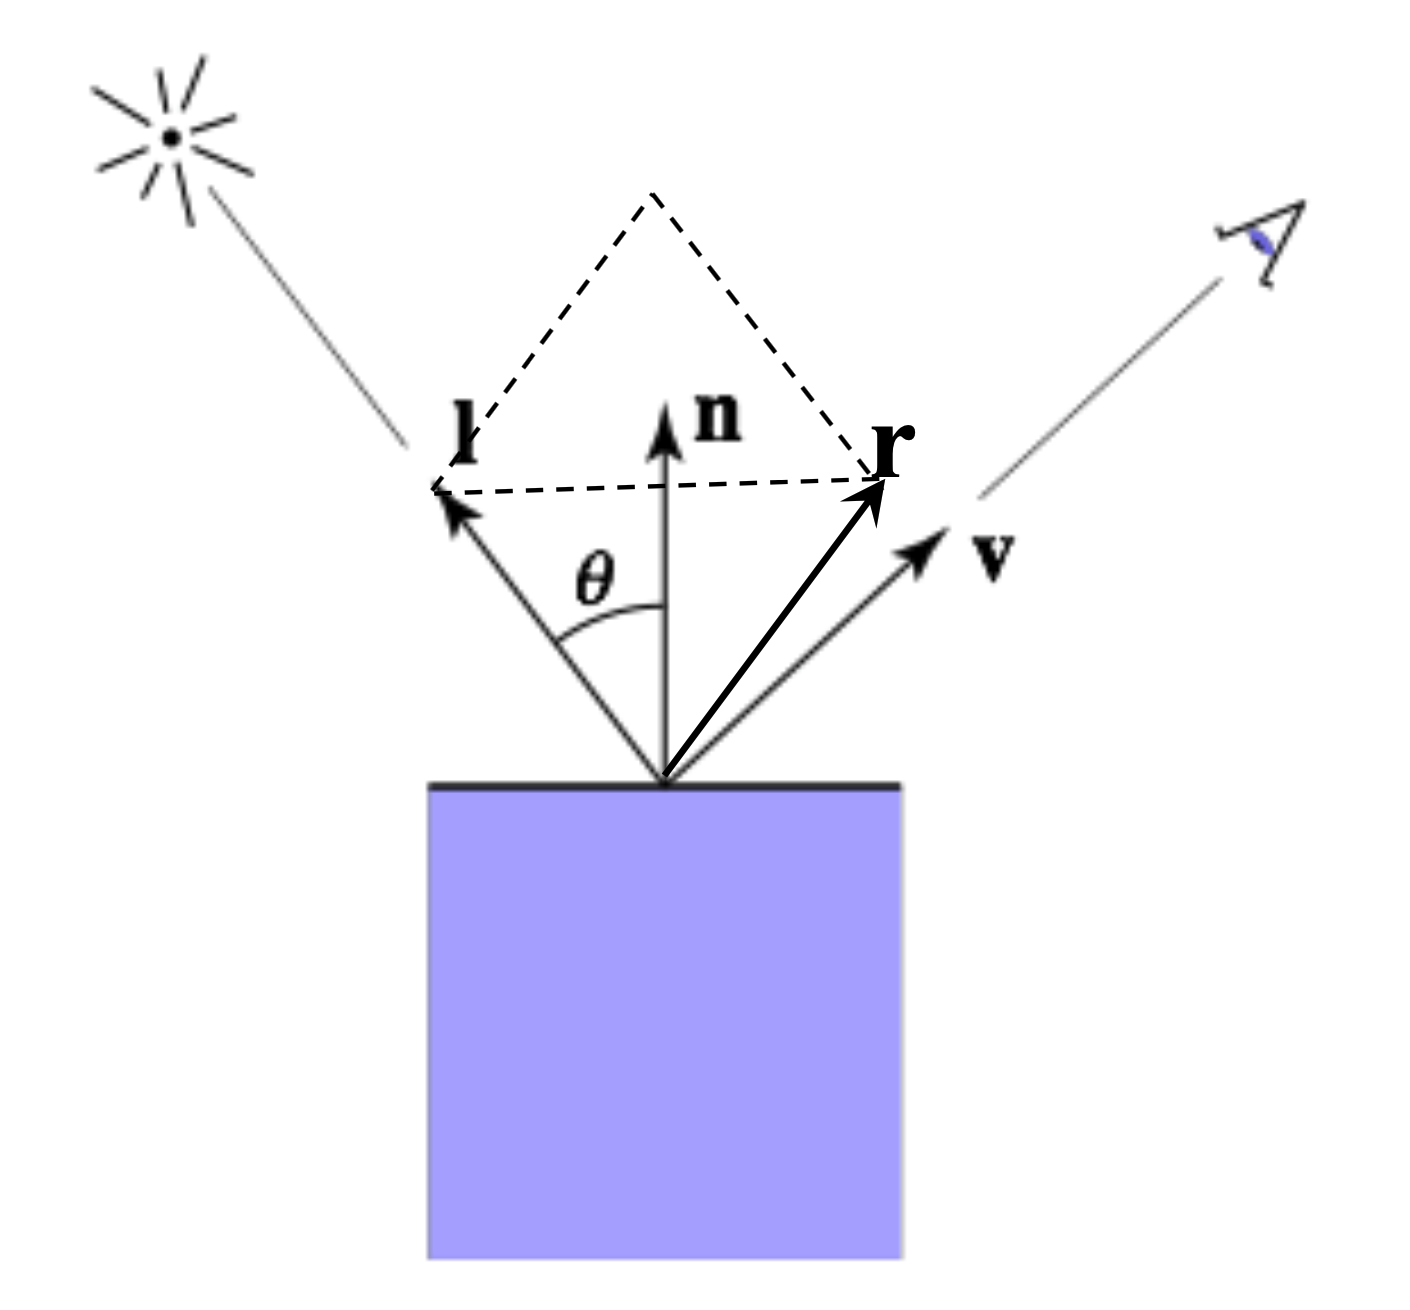
\includegraphics[width=0.5\textwidth]{figs/mirror reflection}
	\caption{\label{mirror reflection} Mirror reflection illustration}
\end{figure}

\subsection{Phong Specular Shading}
With a perfect mirror, only when $\br = \bv$ in Figure \ref{mirror reflection} would the eye see light. In real world, this rarely is the case and we wish to model a common imperfect mirror where there will be some light being reflected to directions around $\br$. Phong specular shading aims to model reflections from this imperfect mirror - the intensity would depend on the view direction, and is bright near mirror configuration: 
\begin{equation}
	k_s \circ I_s (\bv \cdot \br)^{shiny}
\end{equation}
where $k_s$ is yet another set of coefficient guarding three channels, $I_s$ is the three channel intensity (distance decay taken into account already), and $shiny$ is a constant hyper-parameter raised to exponent dictating how fast the $(\bv \cdot \br)$ diminishes to $0$. A large $shiny$ exponent will make the surface more glossy, while a smaller one will make the surface more matte-looking. 

\subsection{Blinn(-Phong) Specular Shading}
Blinn specular shading is just another formulation.\footnote{This very simple and widely used model for specular highlights was proposed by Phong (Phong, 1975) and later updated by Blinn (J. F. Blinn, 1976) to the form most commonly used today.} Figure \ref{blinn} illustrate what we want to calculate. Let's call the point of reflection $\bo$, then in Phong model, we used $\br\bo\bv$ to model the angle and here in Blinn we will be using $\bh\bo\bn$ instead. Notice that however, we do need to calculate an extra vector $\bh$ that is the normalized sum of $\bv$ and $\bl$, i.e. 
\begin{equation}
	\mathbf{h}=\frac{\mathbf{v}+1}{\|\mathbf{v}+1\|}
\end{equation}
The specular reflected intensities can be calculated
\begin{equation}
	L = k_s \circ I \max \{ 0, \bn \cdot \bh \}^p
\end{equation}
where $k_s$ is our guarding coefficients, $I$ is the intensity at the point of reflection (distance decay taken into account already), $p$ is something similar to $shiny$ from before. Again, a larger $p$ means a shinier surface and  a smaller one means more matte-looking. 

\begin{figure}
	\centering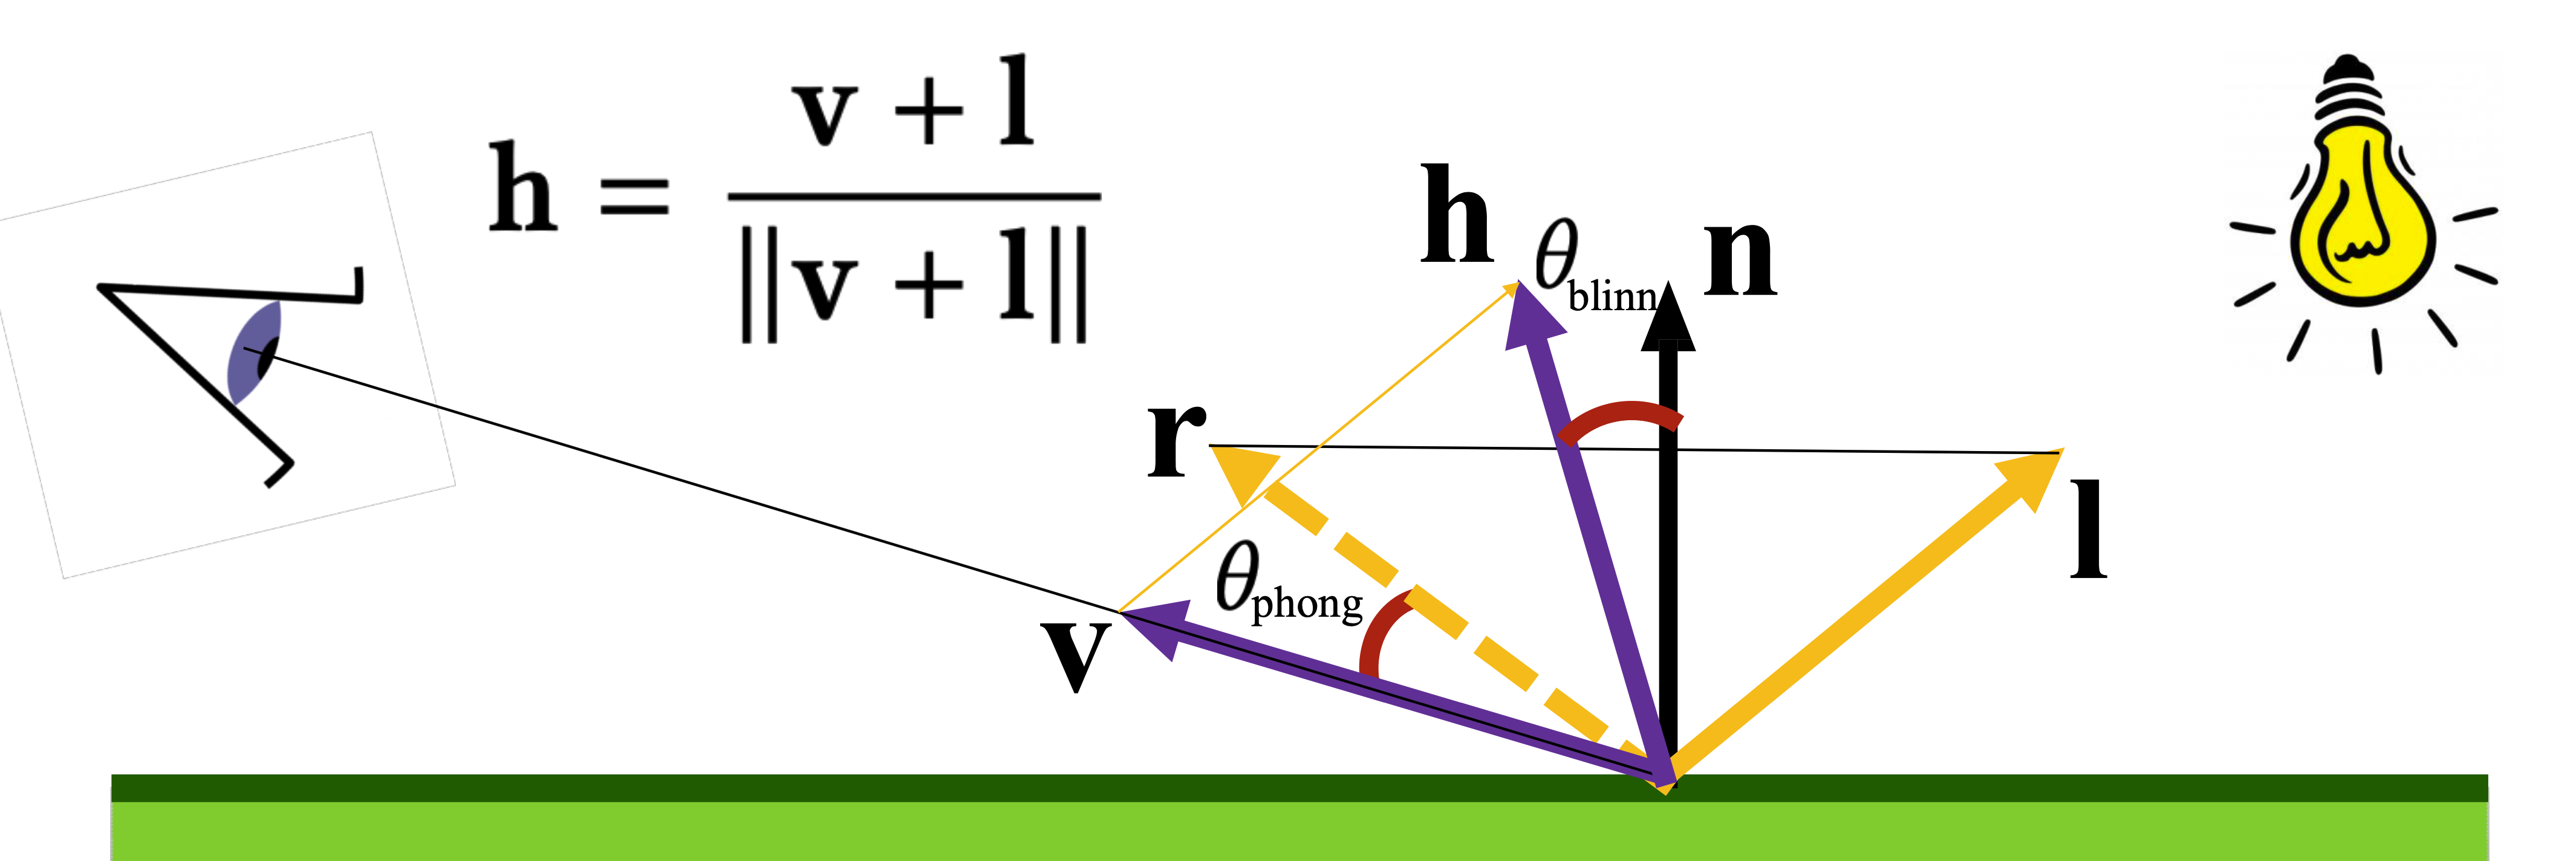
\includegraphics[width=0.8\textwidth]{figs/blinn}
	\caption{\label{blinn} Blinn Specular Shading and Phong Specular Shading.}
\end{figure}

\subsection{Local Illumination}
\begin{itemize}
	\item Usually include ambient, diffuse, Phong\unsure{isn't this Blinn??} in one model
	\begin{equation}
		\begin{aligned}
			L &=L_{a}+L_{d}+L_{s} \\
			&=k_{a} I_{a}+k_{d}\left(I / r^{2}\right) \max (0, \mathbf{n} \cdot \mathbf{l})+k_{s}\left(I / r^{2}\right) \max (0, \mathbf{n} \cdot \mathbf{h})^{p}
		\end{aligned}
	\end{equation}
	\item The final result is the sum over many lights
	\begin{align}
		L
		&= L_{a}+\sum_{i=1}^{N}\left[\left(L_{d}\right)_{i}+\left(L_{s}\right)_{i}\right] \\
		&=k_{a} I_{a}+\sum_{i=1}^{N}\left[k_{d}\left(I_{i} / r_{i}^{2}\right) \max \left(0, \mathbf{n} \cdot \mathbf{l}_{i}\right)+
		k_{s}\left(I_{i} / r_{i}^{2}\right) \max \left(0, \mathbf{n} \cdot \mathbf{h}_{i}\right)^{p}\right]
	\end{align}
\end{itemize}

\subsection{Ray Tracing Template}
{\center 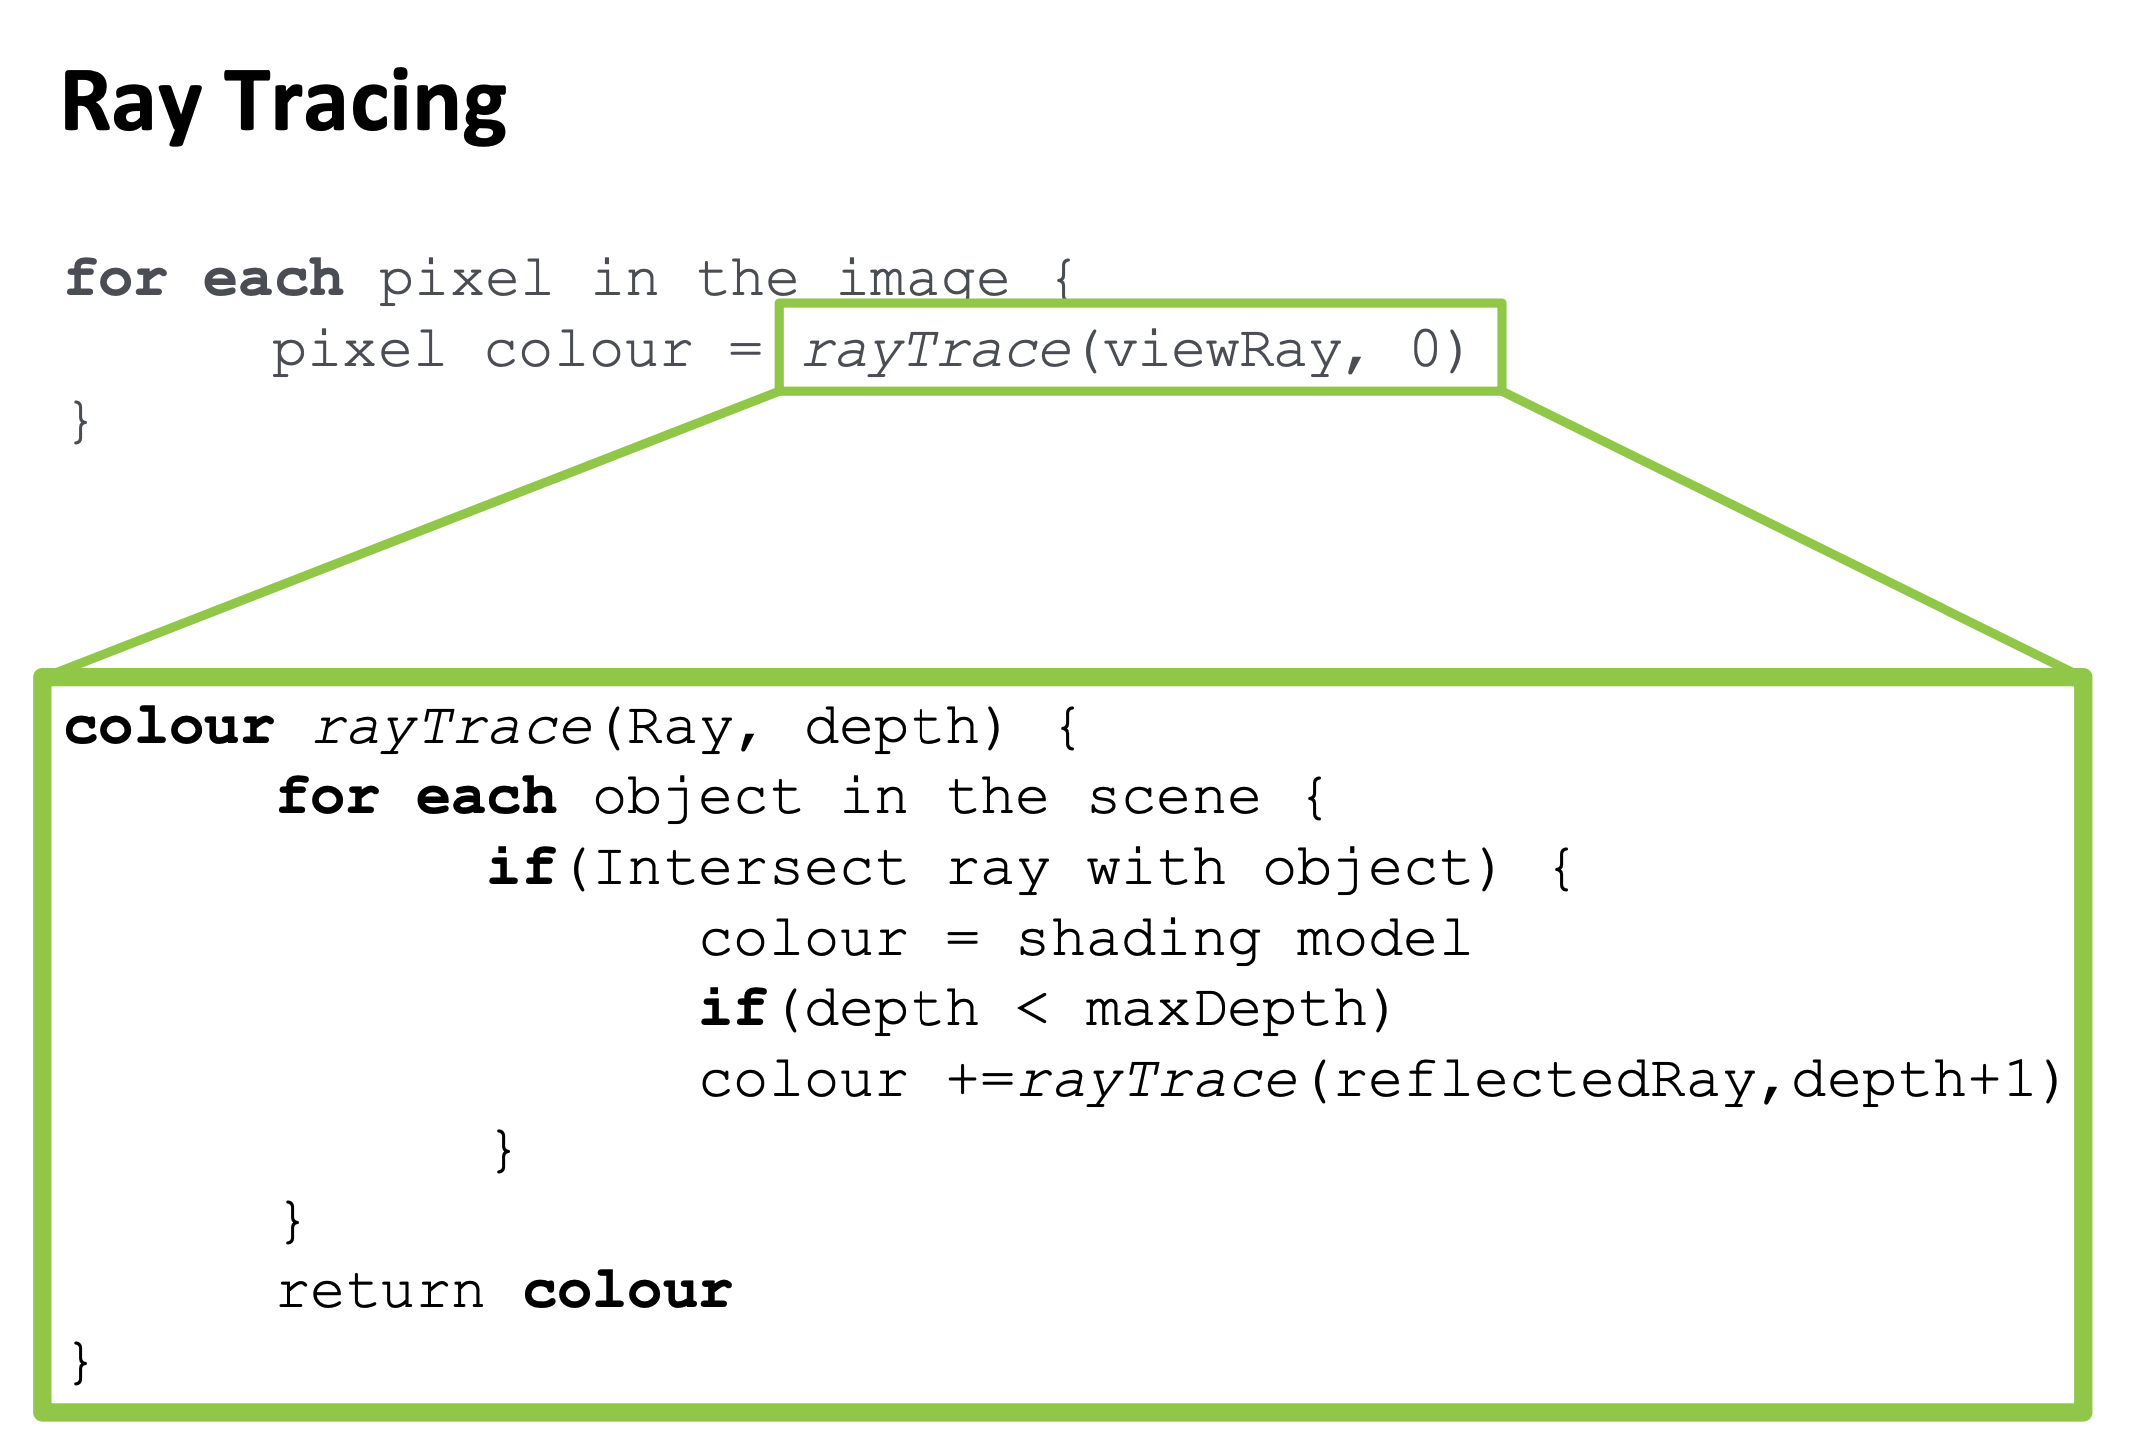
\includegraphics[width=1.0\textwidth]{figs/ray trace}}

\subsection{Refraction - Snell's Law}
Consider a surface with normal $\bn$, with incoming light vector $-\bl$ (so $\bl$ is pointing into the surface), call $\theta_l := \bn\bo\bl$. Suppose the refracted light vector is named $\bt$ with $theta_t:= \bt\bo (-\bn )$, then Snell's Law states that
\begin{equation}
	c_l \sin\theta_l = c_t \sin \theta_t
\end{equation}
We can derive that our unknown of interest $\bt$ is such that 
\begin{equation}
	\bt = -\frac{c_l}{c_t}\bl + \frac{c_l}{c_t} \cos(\theta_l) \bn - \cos (\theta_t ) \bn
\end{equation}
To take refractions into account, we just need to slightly modify the ray tracing template presented previously. Namely, we will need to add 
\begin{verbatim}
	...
	colour += raytrace(reflectedRay, depth+1)
	colour += raytrace(refractedRay, depth+1)
\end{verbatim}















\end{document}
